\section{Phân loại Đa phương thức với CLIP}\label{sec:multimodal}

\subsection{Giới thiệu}
Phân loại đa phương thức (Multimodal Classification) là bài toán nhận dạng và phân loại dữ liệu từ nhiều nguồn thông tin khác nhau, trong đó phổ biến nhất là sự kết hợp giữa \textbf{hình ảnh} và \textbf{văn bản}. Khác với phân loại đơn phương thức truyền thống (chỉ dùng ảnh hoặc chỉ dùng text), phương pháp đa phương thức có khả năng tận dụng thông tin bổ sung từ nhiều modality để cải thiện độ chính xác.

Trong phần này, chúng tôi thực hiện so sánh \textbf{ba phương pháp} phân loại đa phương thức trên tập dữ liệu COCO (Common Objects in Context), sử dụng mô hình CLIP (Contrastive Language-Image Pre-training) từ OpenAI:

\begin{enumerate}
    \item \textbf{Zero-shot Classification}: Phân loại trực tiếp mà không cần huấn luyện thêm.
    \item \textbf{Few-shot Classification (Frozen Backbone)}: Tinh chỉnh đầu phân loại với số lượng mẫu nhỏ (k=1,5,10,20), giữ nguyên trọng số của mạng nền CLIP.
    \item \textbf{Full Fine-Tuning (Unfrozen Backbone)}: Tinh chỉnh toàn bộ mô hình CLIP với lượng dữ liệu lớn hơn (100 samples/class).
\end{enumerate}

\subsection{Tập dữ liệu COCO 2017}\label{subsec:coco-dataset}

\subsubsection{Giới thiệu về COCO}
COCO (Common Objects in Context) là một trong những tập dữ liệu chuẩn quốc tế quan trọng nhất cho các bài toán thị giác máy tính, bao gồm:
\begin{itemize}
    \item \textbf{Object Detection} (Phát hiện đối tượng)
    \item \textbf{Instance Segmentation} (Phân đoạn thực thể)
    \item \textbf{Image Captioning} (Mô tả ảnh)
    \item \textbf{Multimodal Classification} (Phân loại đa phương thức)
\end{itemize}

Tập dữ liệu gốc chứa \textbf{80 categories} phổ biến trong đời sống hàng ngày, từ con người, phương tiện, động vật đến đồ vật gia dụng. Mỗi ảnh trong COCO đi kèm với:
\begin{itemize}
    \item \textbf{Annotations}: Bounding boxes, segmentation masks
    \item \textbf{Captions}: 5 câu mô tả tiếng Anh cho mỗi ảnh
    \item \textbf{Category labels}: Nhãn phân loại đối tượng
\end{itemize}

\subsubsection{Xử lý và Lọc Dữ liệu}
Trong thực nghiệm này, chúng tôi sử dụng phiên bản COCO 2017 từ Kaggle\footnote{Kaggle COCO Dataset: \url{https://www.kaggle.com/datasets/awsaf49/coco-2017-dataset}}. Quy trình xử lý dữ liệu bao gồm:

\begin{enumerate}
    \item \textbf{Kết hợp train và validation splits}: Gộp cả train2017 và val2017 để tăng số lượng mẫu.
    \item \textbf{Lọc categories thiếu dữ liệu}: Loại bỏ các categories có ít hơn 100 samples để đảm bảo chất lượng huấn luyện.
    \item \textbf{Primary category assignment}: Với mỗi ảnh chứa nhiều đối tượng, chọn đối tượng có diện tích lớn nhất làm category chính.
    \item \textbf{Caption extraction}: Lấy caption đầu tiên cho mỗi ảnh làm thông tin văn bản.
\end{enumerate}

Sau khi xử lý, tập dữ liệu cuối cùng có các thông số sau:

\begin{table}[H]
    \centering
    \caption{Thống kê tập dữ liệu COCO sau xử lý}
    \begin{tabular}{|l|r|}
        \hline
        \textbf{Thuộc tính} & \textbf{Giá trị} \\
        \hline
        Tổng số categories & 43 \\
        \hline
        Tổng số samples & 4,424 \\
        \hline
        Samples per class & 100-103 \\
        \hline
        Training set (80\%) & 3,539 \\
        \hline
        Test set (20\%) & 885 \\
        \hline
        Modality & Image + Text (caption) \\
        \hline
    \end{tabular}
    \label{tab:coco-stats}
\end{table}

\textbf{43 categories} được giữ lại bao gồm: person, dog, bowl, bench, toilet, motorcycle, boat, bed, giraffe, car, zebra, chair, airplane, umbrella, bus, cow, dining table, teddy bear, couch, horse, bird, elephant, sheep, clock, train, bicycle, truck, oven, refrigerator, pizza, stop sign, kite, sink, sandwich, cat, fire hydrant, tv, traffic light, bear, suitcase, laptop, surfboard, vase.

\subsection{Kiến trúc CLIP}\label{subsec:clip-architecture}

\subsubsection{Tổng quan về CLIP}
CLIP (Contrastive Language-Image Pre-training) là mô hình đột phá từ OpenAI, được giới thiệu năm 2021\cite{radford2021learning}. Điểm đặc biệt của CLIP là khả năng học biểu diễn chung (joint representation) cho cả hình ảnh và văn bản thông qua huấn luyện contrastive trên \textbf{400 triệu cặp image-text} từ internet.

\begin{figure}[H]
    \centering
    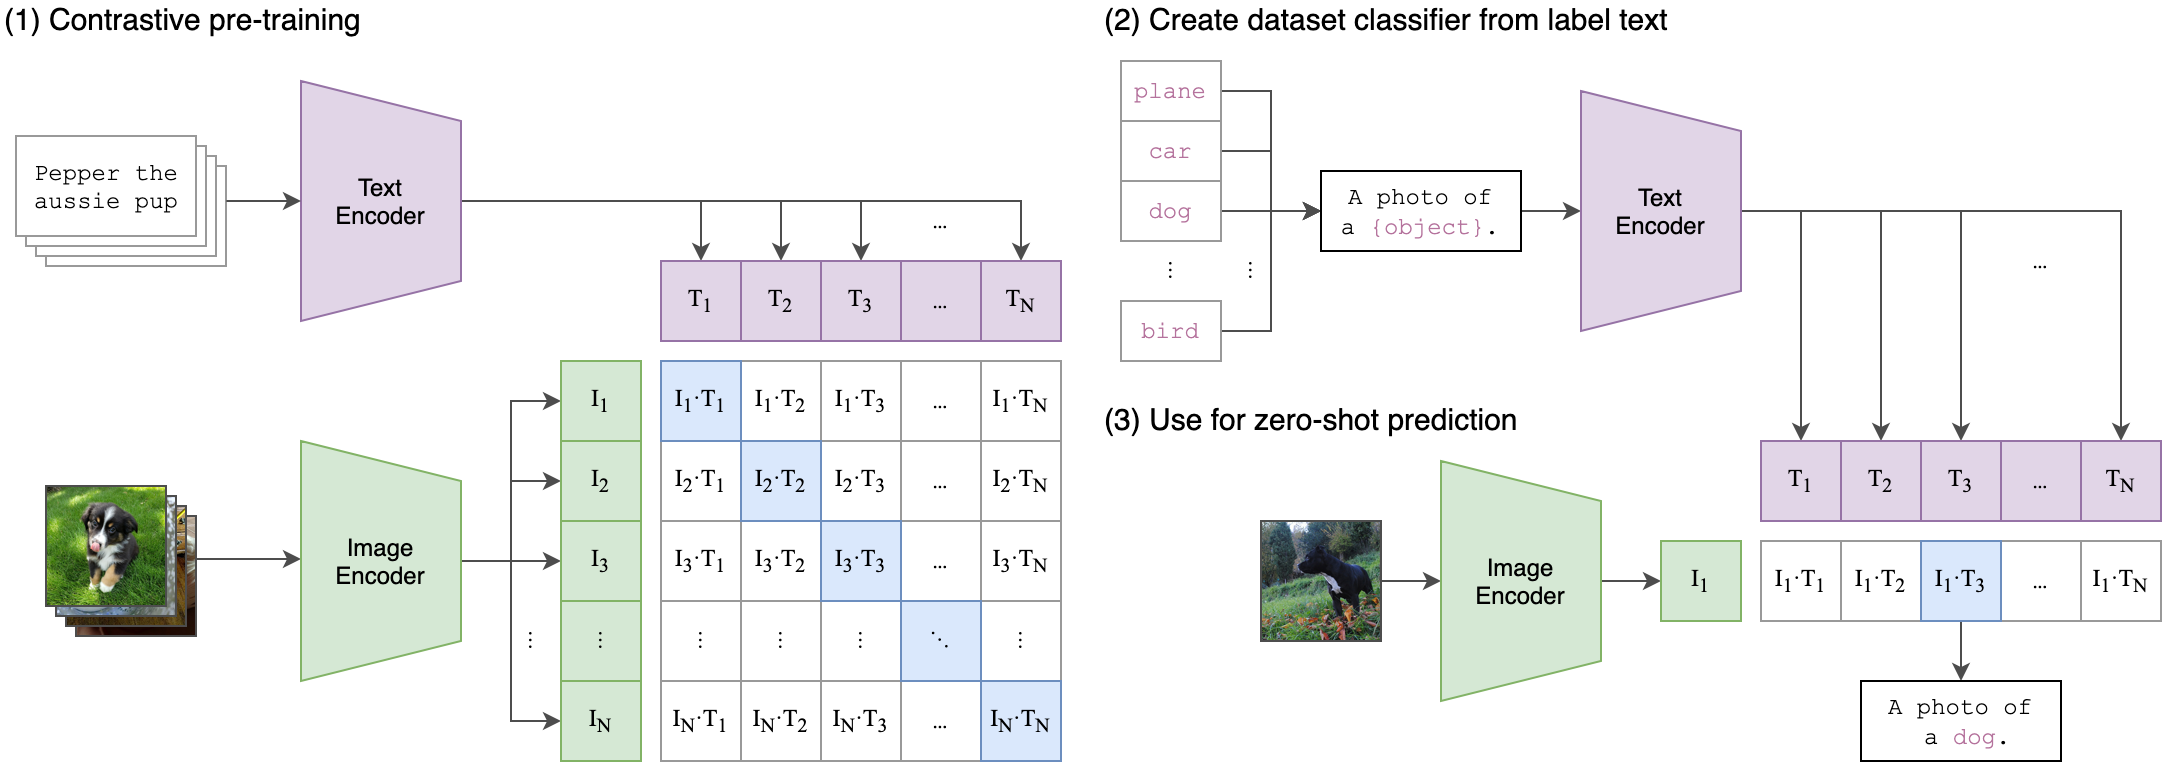
\includegraphics[width=0.95\textwidth]{Images/clip_architecture.png}

    \vspace{0.5cm}
    \caption{Kiến trúc CLIP: Vision Encoder và Text Encoder được huấn luyện để tạo ra biểu diễn tương đồng cho các cặp ảnh-văn bản phù hợp\protect\footnotemark}
    \label{fig:clip-architecture}
\end{figure}
\footnotetext{Nguồn: OpenAI CLIP repository - \url{https://github.com/openai/CLIP}}

\subsubsection{Các thành phần chính}
CLIP bao gồm hai encoder hoạt động song song:

\paragraph{Vision Encoder}
Sử dụng kiến trúc \textbf{Vision Transformer (ViT)} với patch size 32x32. Mô hình chia ảnh đầu vào thành các patches nhỏ, sau đó xử lý chúng như một chuỗi tokens tương tự như trong NLP.

\begin{itemize}
    \item \textbf{Input}: Ảnh RGB kích thước $224 \times 224$ pixels
    \item \textbf{Patch embedding}: Chia thành $7 \times 7 = 49$ patches
    \item \textbf{Transformer layers}: 12 layers với multi-head attention
    \item \textbf{Output}: Image embedding vector $\in \mathbb{R}^{512}$
\end{itemize}

\paragraph{Text Encoder}
Sử dụng kiến trúc \textbf{Transformer} để mã hóa câu văn bản thành vector đặc trưng.

\begin{itemize}
    \item \textbf{Input}: Text sequence (max 77 tokens)
    \item \textbf{Tokenization}: Byte-Pair Encoding (BPE)
    \item \textbf{Transformer layers}: 12 layers với causal attention
    \item \textbf{Output}: Text embedding vector $\in \mathbb{R}^{512}$
\end{itemize}

\subsubsection{Contrastive Learning}
CLIP được huấn luyện với mục tiêu contrastive: tối đa hóa cosine similarity giữa các cặp (image, text) đúng và tối thiểu hóa similarity giữa các cặp không khớp. Hàm loss được định nghĩa:

\begin{equation}
    \mathcal{L}_{\text{CLIP}} = \frac{1}{2}\left(\mathcal{L}_{\text{I2T}} + \mathcal{L}_{\text{T2I}}\right)
\end{equation}

Trong đó:
\begin{itemize}
    \item $\mathcal{L}_{\text{I2T}}$: Cross-entropy loss từ image sang text
    \item $\mathcal{L}_{\text{T2I}}$: Cross-entropy loss từ text sang image
\end{itemize}

\subsubsection{Tại sao CLIP phù hợp cho Multimodal Classification?}
\begin{enumerate}
    \item \textbf{Pre-trained trên dữ liệu đa dạng}: 400M cặp image-text từ internet.
    \item \textbf{Zero-shot capability}: Có thể phân loại các class chưa từng thấy trong quá trình huấn luyện.
    \item \textbf{Joint embedding space}: Biểu diễn ảnh và text trong cùng một không gian vector.
    \item \textbf{Transfer learning friendly}: Dễ dàng fine-tune cho các tác vụ downstream.
\end{enumerate}

\subsection{Ba Phương pháp So sánh}\label{subsec:three-methods}

\subsubsection{Zero-Shot Classification}\label{subsubsec:zero-shot}

\paragraph{Khái niệm}
Zero-shot classification là phương pháp phân loại \textbf{không cần huấn luyện thêm} (no additional training). Mô hình CLIP pretrained được sử dụng trực tiếp để phân loại các ảnh bằng cách so sánh chúng với các text prompts tương ứng với mỗi category.

\paragraph{Cơ chế hoạt động}
\begin{enumerate}
    \item \textbf{Tạo text prompts}: Với mỗi category $c$, tạo prompt theo template: \texttt{"a photo of a \{category\}"}

    Ví dụ:
    \begin{itemize}
        \item Category "person" → \texttt{"a photo of a person"}
        \item Category "car" → \texttt{"a photo of a car"}
    \end{itemize}

    \item \textbf{Encode image và text}:
    \begin{align}
        \mathbf{v}_{\text{img}} &= \text{VisionEncoder}(\text{image}) \\
        \mathbf{v}_{\text{text}}^{(i)} &= \text{TextEncoder}(\text{prompt}_i), \quad i=1,\ldots,C
    \end{align}

    \item \textbf{Tính similarity scores}:
    \begin{equation}
        s_i = \cos(\mathbf{v}_{\text{img}}, \mathbf{v}_{\text{text}}^{(i)}) = \frac{\mathbf{v}_{\text{img}} \cdot \mathbf{v}_{\text{text}}^{(i)}}{\|\mathbf{v}_{\text{img}}\| \|\mathbf{v}_{\text{text}}^{(i)}\|}
    \end{equation}

    \item \textbf{Dự đoán category}:
    \begin{equation}
        \hat{y} = \arg\max_{i} \, \text{softmax}(s_i / \tau)
    \end{equation}

    Trong đó $\tau$ là temperature parameter (thường = 0.01).
\end{enumerate}

\paragraph{Ưu điểm}
\begin{itemize}
    \item Không cần dữ liệu huấn luyện
    \item Thời gian inference nhanh (không có training phase)
    \item Có thể mở rộng sang các class mới ngay lập tức
    \item Tận dụng tối đa knowledge từ pretrained model
\end{itemize}

\paragraph{Nhược điểm}
\begin{itemize}
    \item Không customize được cho dataset cụ thể
    \item Performance bị giới hạn bởi pretrained knowledge
    \item Có thể kém hiệu quả với domain-specific tasks
\end{itemize}

\paragraph{Cấu hình thực nghiệm}
\begin{table}[H]
    \centering
    \caption{Thông số Zero-shot Classification}
    \begin{tabular}{|l|l|}
        \hline
        \textbf{Tham số} & \textbf{Giá trị} \\
        \hline
        Model & openai/clip-vit-base-patch32 \\
        \hline
        Training data & 0 samples \\
        \hline
        Trainable parameters & 0 (all frozen) \\
        \hline
        Training time & 0s \\
        \hline
        Prompt template & "a photo of a \{category\}" \\
        \hline
        Temperature $\tau$ & 0.01 \\
        \hline
    \end{tabular}
    \label{tab:zero-shot-config}
\end{table}

\subsubsection{Few-Shot Classification (Frozen Backbone)}\label{subsubsec:few-shot}

\paragraph{Khái niệm}
Few-shot classification là phương pháp huấn luyện mô hình với \textbf{số lượng mẫu rất nhỏ} cho mỗi class (thường từ 1-20 samples). Trong phương pháp này, backbone CLIP được \textbf{đóng băng} (frozen), chỉ có classification head được huấn luyện.

\paragraph{Kiến trúc}
Mô hình bao gồm hai phần chính:

\begin{enumerate}
    \item \textbf{CLIP Encoder (FROZEN)}:
    \begin{itemize}
        \item Vision Encoder: xử lý ảnh → image embedding
        \item Text Encoder: xử lý caption → text embedding
        \item Tất cả trọng số của CLIP đều \texttt{requires\_grad=False}
    \end{itemize}

    \item \textbf{Classification Head (TRAINABLE)}:
    \begin{itemize}
        \item Input: Concatenation của image embedding và text embedding
        \item Architecture: 2-layer MLP
        \item Layer 1: Linear($512 \times 2 = 1024$, 512) + ReLU + Dropout(0.1)
        \item Layer 2: Linear(512, num\_classes)
        \item Output: Logits cho 43 categories
    \end{itemize}
\end{enumerate}

\begin{minted}[linenos, breaklines, fontsize=\small]{python}
class CLIPClassifier(nn.Module):
    def __init__(self, clip_model, num_classes, freeze_backbone=True):
        super().__init__()
        self.clip = clip_model

        # Đóng băng CLIP backbone
        if freeze_backbone:
            for param in self.clip.parameters():
                param.requires_grad = False

        # Classification head (trainable)
        hidden_size = self.clip.config.projection_dim  # 512
        self.classifier = nn.Sequential(
            nn.Linear(hidden_size * 2, hidden_size),
            nn.ReLU(),
            nn.Dropout(0.1),
            nn.Linear(hidden_size, num_classes)
        )

    def forward(self, input_ids, attention_mask, pixel_values):
        outputs = self.clip(input_ids, attention_mask, pixel_values)
        combined = torch.cat([outputs.image_embeds,
                             outputs.text_embeds], dim=1)
        return self.classifier(combined)
\end{minted}

\paragraph{Cấu hình huấn luyện}
Chúng tôi thực nghiệm với \textbf{4 giá trị k khác nhau}: k=1, 5, 10, 20 samples per class.

\begin{table}[H]
    \centering
    \caption{Thông số Few-shot Classification}
    \begin{tabular}{|l|l|l|l|l|}
        \hline
        \textbf{Tham số} & \textbf{1-shot} & \textbf{5-shot} & \textbf{10-shot} & \textbf{20-shot} \\
        \hline
        Training samples & 43 & 215 & 430 & 860 \\
        \hline
        Samples/class & 1 & 5 & 10 & 20 \\
        \hline
        Epochs & 20 & 20 & 10 & 10 \\
        \hline
        Learning rate & 1e-4 & 1e-4 & 5e-5 & 5e-5 \\
        \hline
        Batch size & 8 & 8 & 8 & 8 \\
        \hline
        Optimizer & \multicolumn{4}{c|}{AdamW} \\
        \hline
        Trainable params & \multicolumn{4}{c|}{~262K (chỉ classification head)} \\
        \hline
        Frozen params & \multicolumn{4}{c|}{~151M (CLIP backbone)} \\
        \hline
    \end{tabular}
    \label{tab:few-shot-config}
\end{table}

\paragraph{Ưu điểm}
\begin{itemize}
    \item Cải thiện performance với rất ít dữ liệu
    \item Training nhanh (chỉ train head, không train backbone)
    \item Tránh overfitting nhờ freeze pretrained weights
    \item Giữ lại được generalization capability của CLIP
\end{itemize}

\paragraph{Nhược điểm}
\begin{itemize}
    \item Performance bị giới hạn bởi frozen features
    \item Không thể adapt backbone cho domain-specific patterns
    \item Với k quá nhỏ (k=1), performance vẫn rất thấp
\end{itemize}

\subsubsection{Full Fine-Tuning (Unfrozen Backbone)}\label{subsubsec:full-finetune}

\paragraph{Khái niệm}
Full fine-tuning là phương pháp huấn luyện \textbf{toàn bộ mô hình}, bao gồm cả CLIP backbone. Khác với few-shot learning, ở đây tất cả các layers đều có thể cập nhật trọng số (\texttt{requires\_grad=True}).

\paragraph{Điểm khác biệt chính}
\begin{table}[H]
    \centering
    \caption{So sánh Few-shot (Frozen) vs Full Fine-tuning (Unfrozen)}
    \begin{tabular}{|l|l|l|}
        \hline
        \textbf{Aspect} & \textbf{Few-shot (Frozen)} & \textbf{Full Fine-tune (Unfrozen)} \\
        \hline
        Backbone status & \texttt{freeze\_backbone=True} & \texttt{freeze\_backbone=False} \\
        \hline
        Trainable layers & Chỉ classification head & Toàn bộ model \\
        \hline
        Trainable params & ~262K & ~546K \\
        \hline
        Training data & 1-20 samples/class & 100 samples/class \\
        \hline
        Learning rate & 1e-4 hoặc 5e-5 & 2e-5 (thấp hơn) \\
        \hline
        Epochs & 10-20 & 5 (ít hơn) \\
        \hline
        Risk of overfitting & Thấp & Cao hơn \\
        \hline
        Training time & Nhanh (~85-137s) & Chậm hơn (~151s) \\
        \hline
    \end{tabular}
    \label{tab:frozen-vs-unfrozen}
\end{table}

\paragraph{Cấu hình huấn luyện}
\begin{table}[H]
    \centering
    \caption{Thông số Full Fine-Tuning}
    \begin{tabular}{|l|l|}
        \hline
        \textbf{Tham số} & \textbf{Giá trị} \\
        \hline
        Training samples & 3,539 (100 samples/class) \\
        \hline
        Epochs & 5 \\
        \hline
        Learning rate & 2e-5 (thấp để stability) \\
        \hline
        Batch size & 8 \\
        \hline
        Optimizer & AdamW \\
        \hline
        Scheduler & Linear warmup (10\% steps) \\
        \hline
        Trainable params & ~546K (toàn bộ model) \\
        \hline
        freeze\_backbone & False \\
        \hline
    \end{tabular}
    \label{tab:full-finetune-config}
\end{table}

\paragraph{Ưu điểm}
\begin{itemize}
    \item Tiềm năng đạt accuracy cao nhất
    \item Có thể adapt toàn bộ model cho domain-specific task
    \item Học được patterns phức tạp hơn từ dữ liệu
\end{itemize}

\paragraph{Nhược điểm}
\begin{itemize}
    \item Cần nhiều dữ liệu hơn (ít nhất 50-100 samples/class)
    \item Training chậm hơn (train toàn bộ 151M parameters)
    \item Nguy cơ overfitting cao nếu dữ liệu không đủ
    \item Có thể mất đi generalization capability của pretrained model
\end{itemize}

\subsection{Thiết lập Thực nghiệm}\label{subsec:experiment-setup}

\subsubsection{Môi trường và Phần cứng}
\begin{itemize}
    \item \textbf{Platform}: Kaggle Notebook
    \item \textbf{GPU}: Tesla T4 x2 (16GB VRAM mỗi card)
    \item \textbf{Framework}: PyTorch 2.x, Transformers (HuggingFace)
    \item \textbf{Python}: 3.10
\end{itemize}

\subsubsection{Chia tách dữ liệu}
\begin{itemize}
    \item \textbf{Test set}: 20\% (885 samples) - stratified by category
    \item \textbf{Training set}: 80\% (3,539 samples)
    \begin{itemize}
        \item Few-shot: Lấy ngẫu nhiên k samples/class (k=1,5,10,20)
        \item Full fine-tune: Sử dụng toàn bộ 100 samples/class
    \end{itemize}
\end{itemize}

\subsubsection{Metrics đánh giá}
Theo yêu cầu của đề bài (Section 4.4), chúng tôi đánh giá tất cả các phương pháp với các metrics sau:

\begin{enumerate}
    \item \textbf{Accuracy}: Tỷ lệ phân loại đúng tổng thể
    \begin{equation}
        \text{Accuracy} = \frac{\text{Số lượng dự đoán đúng}}{\text{Tổng số mẫu}}
    \end{equation}

    \item \textbf{F1 Score (Macro)}: Trung bình cộng F1 của từng class
    \begin{equation}
        F1_{\text{macro}} = \frac{1}{C}\sum_{i=1}^{C} F1_i
    \end{equation}

    \item \textbf{F1 Score (Weighted)}: Trung bình có trọng số theo số lượng samples
    \begin{equation}
        F1_{\text{weighted}} = \sum_{i=1}^{C} w_i \cdot F1_i, \quad w_i = \frac{n_i}{\sum_j n_j}
    \end{equation}

    \item \textbf{Precision (Macro)}: Độ chính xác trung bình
    \item \textbf{Recall (Macro)}: Độ phủ trung bình
    \item \textbf{Confusion Matrix}: Ma trận nhầm lẫn 43x43
    \item \textbf{Per-class Metrics}: F1, Precision, Recall cho từng category
\end{enumerate}

\subsection{Kết quả và Phân tích}\label{subsec:results}

\subsubsection{So sánh Tổng quan}
Bảng~\ref{tab:overall-comparison} tổng hợp kết quả của tất cả 6 thí nghiệm (1 zero-shot + 4 few-shot + 1 full fine-tuning).

\begin{table}[H]
    \centering
    \caption{So sánh tổng quan: Zero-shot vs Few-shot vs Full Fine-tuning}
    \begin{tabular}{|l|r|l|r|r|r|r|r|}
        \hline
        \textbf{Method} & \textbf{K} & \textbf{Backbone} & \textbf{Acc} & \textbf{F1 Ma} & \textbf{F1 We} & \textbf{Prec} & \textbf{Recall} \\
        \hline
        Zero-Shot & 0 & Frozen & \textbf{0.758} & \textbf{0.741} & \textbf{0.740} & 0.754 & 0.759 \\
        \hline
        1-Shot & 1 & Frozen & 0.162 & 0.106 & 0.106 & 0.189 & 0.161 \\
        \hline
        5-Shot & 5 & Frozen & 0.645 & 0.614 & 0.614 & 0.672 & 0.645 \\
        \hline
        10-Shot & 10 & Frozen & 0.399 & 0.367 & 0.367 & 0.487 & 0.398 \\
        \hline
        20-Shot & 20 & Frozen & 0.652 & 0.616 & 0.615 & 0.671 & 0.652 \\
        \hline
        Full FT & 100 & Unfrozen & 0.644 & 0.602 & 0.600 & \textbf{0.653} & \textbf{0.645} \\
        \hline
    \end{tabular}
    \label{tab:overall-comparison}
\end{table}

\textbf{Chú thích}: Acc = Accuracy, F1 Ma = F1 Macro, F1 We = F1 Weighted, Prec = Precision Macro, FT = Fine-Tuning

\paragraph{Quan sát chính}
\begin{enumerate}
    \item \textbf{Zero-shot đạt kết quả tốt nhất} với accuracy 75.8\%, vượt trội hơn tất cả các phương pháp fine-tuning. Điều này cho thấy CLIP pretrained đã học được biểu diễn rất mạnh cho COCO dataset.

    \item \textbf{1-shot performance cực kỳ thấp} (16.2\%), chứng tỏ 1 sample/class không đủ để học được pattern phân loại.

    \item \textbf{5-shot và 20-shot đạt kết quả tương đương nhau} (~64-65\%), cho thấy diminishing returns khi tăng k từ 5 lên 20.

    \item \textbf{Full fine-tuning không vượt trội} (64.4\%), thậm chí còn kém hơn zero-shot. Dưới góc độ lý thuyết, sự sụt giảm này là minh chứng rõ rệt cho hiện tượng \textbf{"Quên thảm khốc" (Catastrophic Forgetting)}. Khi mở khóa (unfreeze) toàn bộ mạng lưới chứa khoảng 150 triệu tham số và liên tục đẩy đạo hàm cập nhật từ một lượng dữ liệu tập trung quá nhỏ (chỉ 100 mẫu/lớp), mô hình đã tự phá vỡ không gian biểu diễn tổng quát mà nó từng tích lũy từ 400 triệu ảnh pre-train. Các trọng số bị "bẻ cong" (bias) thái quá về phía tập phân bố của COCO, hệ quả là mất đi khả năng tổng quát hóa ban đầu.
\end{enumerate}

\subsubsection{Thời gian Huấn luyện và Inference}
\begin{table}[H]
    \centering
    \caption{Phân tích thời gian xử lý}
    \begin{tabular}{|l|r|r|}
        \hline
        \textbf{Method} & \textbf{Training Time (s)} & \textbf{Inference Time (s)} \\
        \hline
        Zero-Shot & 0 & 23.5 \\
        \hline
        1-Shot & 108.5 & 5.2 \\
        \hline
        5-Shot & 136.6 & 5.3 \\
        \hline
        10-Shot & 85.0 & 5.3 \\
        \hline
        20-Shot & 113.9 & 5.2 \\
        \hline
        Full Fine-tuning & 150.7 & 5.2 \\
        \hline
    \end{tabular}
    \label{tab:time-analysis}
\end{table}

\textbf{Nhận xét}:
\begin{itemize}
    \item Zero-shot có inference time cao nhất (23.5s) vì phải encode 43 text prompts cho mỗi batch.
    \item Các phương pháp fine-tuning có inference nhanh hơn (~5s) vì chỉ cần forward pass qua classification head.
    \item Training time tăng dần từ few-shot (85-137s) đến full fine-tuning (151s).
\end{itemize}

\subsubsection{Phân tích theo K (Samples per Class)}
Hình~\ref{fig:metrics-vs-k} cho thấy xu hướng thay đổi của accuracy và F1 macro theo số lượng samples per class.

\begin{figure}[H]
    \centering
    \begin{subfigure}[b]{0.48\textwidth}
        \centering
        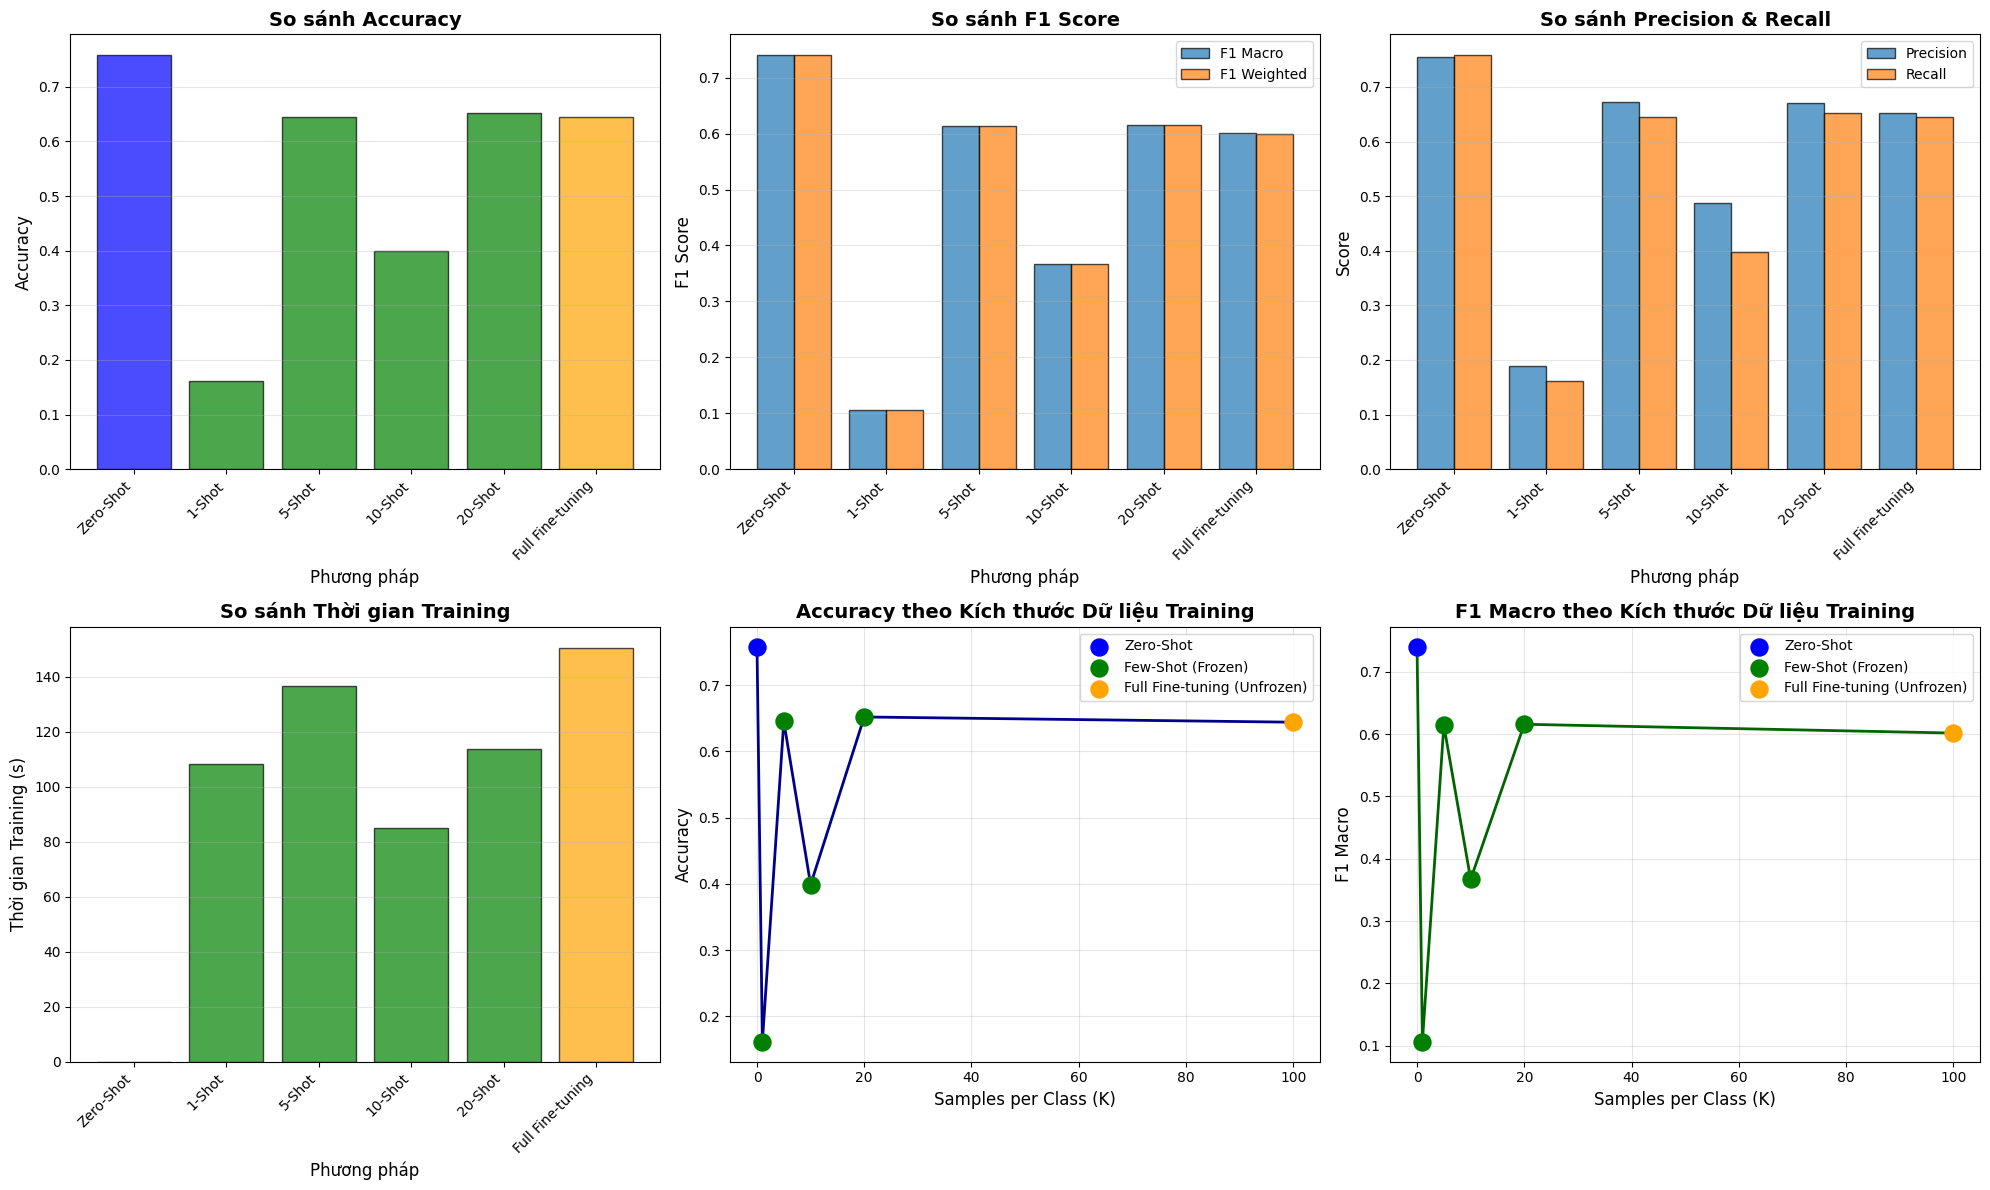
\includegraphics[width=\textwidth]{Images/multimodal_accuracy_vs_k.png}
        \caption{Accuracy theo số lượng samples per class (K)}
        \label{fig:accuracy-vs-k}
    \end{subfigure}
    \hfill
    \begin{subfigure}[b]{0.48\textwidth}
        \centering
        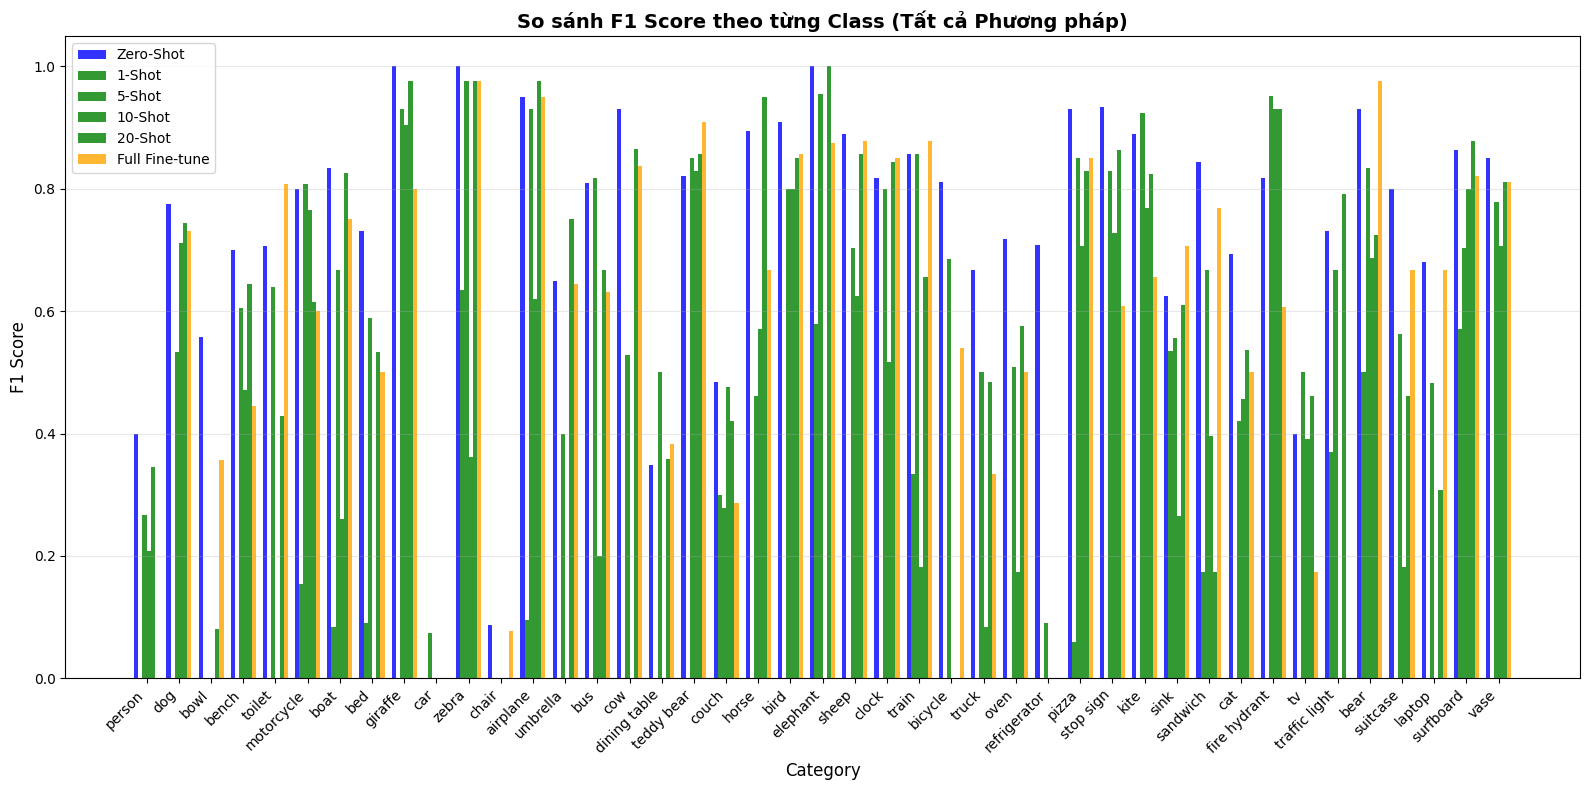
\includegraphics[width=\textwidth]{Images/multimodal_f1_vs_k.png}
        \caption{F1 Macro theo số lượng samples per class (K)}
        \label{fig:f1-vs-k}
    \end{subfigure}

    \vspace{0.5cm}
    \caption{Xu hướng thay đổi metrics theo K. Quan sát: performance tăng mạnh từ k=1 đến k=5, sau đó có diminishing returns.}
    \label{fig:metrics-vs-k}
\end{figure}

\textbf{Quan sát}:
\begin{itemize}
    \item Accuracy tăng mạnh từ k=1 (16\%) lên k=5 (64.5\%)
    \item Từ k=5 trở đi, accuracy gần như không tăng (k=5: 64.5\%, k=20: 65.2\%)
    \item Full fine-tuning (k=100) cũng chỉ đạt 64.4\%, tương đương k=5
    \item Điều này chứng tỏ: \textbf{k=5 đã đủ để đạt performance tốt} với frozen backbone
\end{itemize}

\subsubsection{Confusion Matrices}
Hình~\ref{fig:confusion-matrices} trình bày confusion matrices cho ba phương pháp đại diện: Zero-shot, 5-shot (frozen), và Full fine-tuning (unfrozen).

\begin{figure}[H]
    \centering
    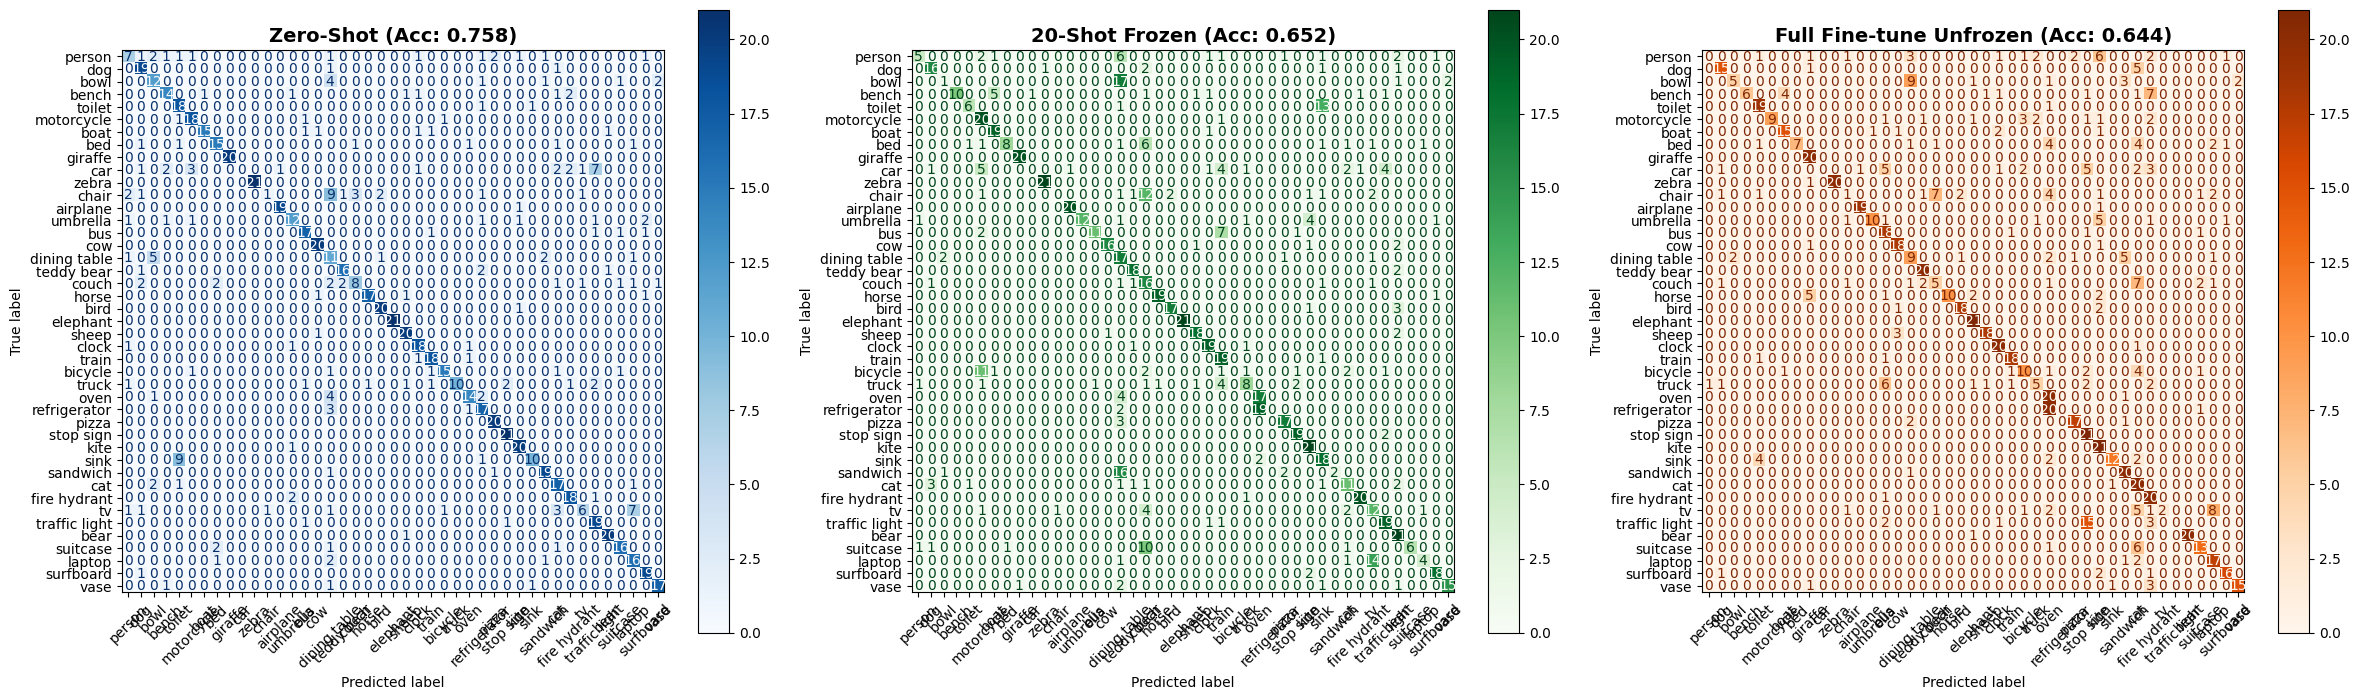
\includegraphics[width=0.95\textwidth]{Images/multimodal_cm_all_three.png}

    \vspace{0.5cm}
    \caption{Confusion matrices cho ba phương pháp (Zero-shot: 75.8\%, 5-Shot: 64.5\%, Full Fine-tune: 64.4\%). Zero-shot có đường chéo chính rõ nhất, cho thấy ít confusion giữa các classes.}
    \label{fig:confusion-matrices}
\end{figure}

\textbf{Phân tích}:
\begin{itemize}
    \item \textbf{Zero-shot}: Đường chéo chính rất nổi bật, ít confusion giữa các classes. Cho thấy CLIP pretrained phân biệt tốt các categories COCO.

    \item \textbf{5-shot}: Có một số confusion tăng lên so với zero-shot, đặc biệt ở các classes tương tự nhau (ví dụ: chair vs couch, car vs truck).

    \item \textbf{Full fine-tuning}: Tương tự 5-shot, không cải thiện đáng kể về confusion patterns.
\end{itemize}

\subsubsection{Per-class Performance}
Phân tích chi tiết F1 score của từng category (Hình~\ref{fig:per-class-f1}) cho thấy:

\begin{figure}[H]
    \centering
    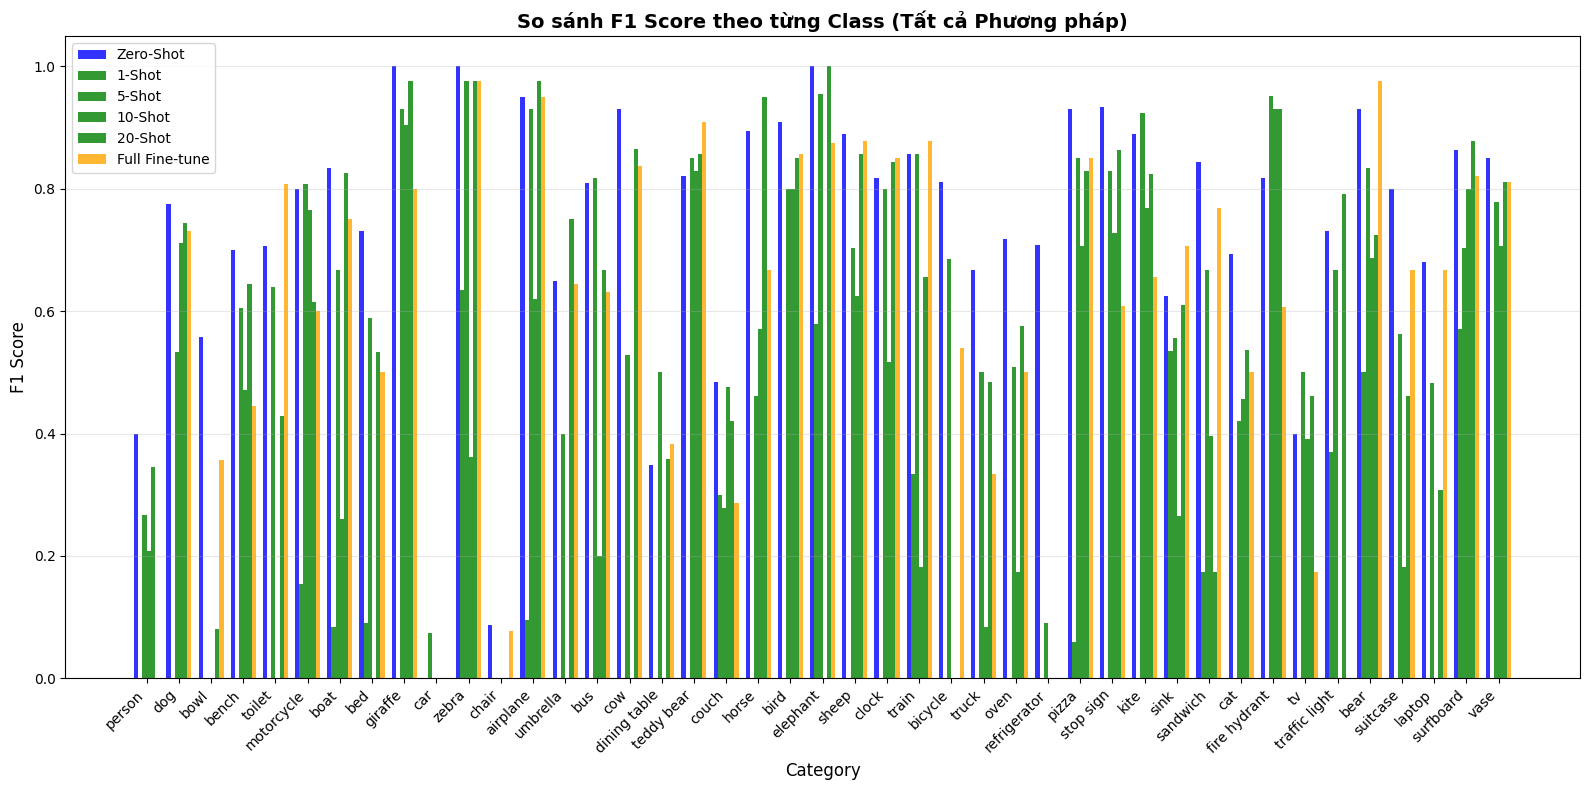
\includegraphics[width=0.95\textwidth]{Images/multimodal_per_class_f1.png}

    \vspace{0.5cm}
    \caption{So sánh F1 score theo từng category. Top performers: giraffe, zebra, elephant. Challenging: chair, person, bowl.}
    \label{fig:per-class-f1}
\end{figure}

\paragraph{Top-performing classes (F1 > 0.9)}
\begin{itemize}
    \item \textbf{giraffe}, \textbf{zebra}, \textbf{elephant}: Động vật có đặc điểm ngoại hình độc nhất
    \item \textbf{airplane}, \textbf{train}: Phương tiện lớn, dễ phân biệt
    \item \textbf{stop sign}, \textbf{pizza}: Có pattern rõ ràng
\end{itemize}

\paragraph{Challenging classes (F1 < 0.5)}
\begin{itemize}
    \item \textbf{chair}: Bị nhầm với bench, couch do cùng là đồ nội thất
    \item \textbf{person}: Xuất hiện trong nhiều context khác nhau
    \item \textbf{bowl}, \textbf{cup}: Nhỏ, khó phân biệt trong ảnh
\end{itemize}

\subsection{Kết luận}\label{subsec:conclusion}

\subsubsection{Tổng kết Kết quả}
Qua thực nghiệm so sánh ba phương pháp phân loại đa phương thức trên COCO dataset, chúng tôi rút ra các kết luận sau:

\begin{enumerate}
    \item \textbf{Zero-shot CLIP cực kỳ mạnh} cho COCO dataset (75.8\% accuracy), vượt trội hơn cả fine-tuning. Điều này chứng tỏ CLIP pretrained đã học được biểu diễn tốt cho các object categories phổ biến.

    \item \textbf{Few-shot learning hiệu quả với ít dữ liệu}. Chỉ với 5 samples/class, model đã đạt 64.5\% accuracy, cải thiện đáng kể so với 1-shot (16.2\%).

    \item \textbf{Diminishing returns khi tăng k}: Performance gần như không thay đổi từ k=5 đến k=20, cho thấy k=5 đã đủ để học được pattern cơ bản.

    \item \textbf{Hệ lụy của Full Fine-tuning trên dữ liệu nhỏ}: Việc unfreeze toàn bộ mạng backbone khổng lồ trên lượng dữ liệu ít ỏi không mang lại cải thiện. Thay vào đó, nó gây ra hiện tượng \textbf{"Quên thảm khốc" (Catastrophic Forgetting)}, khiến mô hình đánh mất năng lực tổng quát hóa nguyên bản và rơi vào trạng thái quá khớp (overfitting) cục bộ.
\end{enumerate}

\subsubsection{Trade-offs giữa các Phương pháp}

\begin{table}[H]
    \centering
    \caption{So sánh Trade-offs}
    \begin{tabular}{|l|l|l|l|}
        \hline
        \textbf{Tiêu chí} & \textbf{Zero-Shot} & \textbf{Few-Shot} & \textbf{Full Fine-tune} \\
        \hline
        Training data & Không cần & Ít (5-20/class) & Nhiều (100+/class) \\
        \hline
        Training time & 0s & Phút & Giờ \\
        \hline
        Accuracy & Tốt (75.8\%) & Khá (64.5\%) & Khá (64.4\%) \\
        \hline
        Resource cost & Thấp & Trung bình & Cao \\
        \hline
        Deployment speed & Tức thì & Nhanh & Chậm \\
        \hline
        Customization & Không & Có hạn & Toàn diện \\
        \hline
        Overfitting risk & Không có & Thấp & Cao \\
        \hline
    \end{tabular}
    \label{tab:tradeoffs}
\end{table}

\subsubsection{Khuyến nghị Sử dụng}

\paragraph{Khi nào dùng Zero-shot?}
\begin{itemize}
    \item Không có dữ liệu labeled
    \item Cần triển khai nhanh, không có thời gian training
    \item Task gần với CLIP pretraining (object recognition trên ảnh tự nhiên)
    \item Cần phân loại các classes mới liên tục
\end{itemize}

\paragraph{Khi nào dùng Few-shot (Frozen)?}
\begin{itemize}
    \item Có ít dữ liệu labeled (5-20 samples/class)
    \item Muốn cải thiện performance so với zero-shot
    \item Thời gian training giới hạn (vài phút)
    \item Muốn giữ lại generalization capability của CLIP
\end{itemize}

\paragraph{Khi nào dùng Full Fine-tuning (Unfrozen)?}
\begin{itemize}
    \item Có nhiều dữ liệu labeled (100+ samples/class)
    \item Task khác xa CLIP pretraining (medical images, satellite imagery, etc.)
    \item Có GPU và thời gian để train toàn bộ model
    \item Zero-shot và few-shot không đạt yêu cầu
\end{itemize}

\subsubsection{Hướng Phát triển}
Một số hướng cải thiện tiềm năng:
\begin{enumerate}
    \item \textbf{Prompt engineering}: Thay vì chỉ sử dụng template đơn giản \texttt{"a photo of a \{category\}"}, có thể thử các dạng prompt phong phú hơn nhằm tận dụng tối đa năng lực ngôn ngữ của CLIP để nâng cao hiệu năng Zero-shot. Ví dụ:
    \begin{itemize}
        \item \texttt{"a photo of a \{category\}, a type of animal/vehicle/object"} (cung cấp ngữ cảnh siêu phạm trù)
        \item \texttt{"a clear photo of \{category\} in natural lighting"} (mô tả điều kiện chụp)
        \item \textbf{Prompt Ensembling}: Kết hợp dự đoán từ nhiều template prompt khác nhau và lấy trung bình vector text embedding, thay vì chỉ dùng một template duy nhất. Phương pháp này được OpenAI sử dụng trong bài báo gốc của CLIP và cho thấy cải thiện đáng kể so với single-template.
    \end{itemize}
    \item \textbf{Data augmentation}: Tăng cường dữ liệu cho few-shot learning
    \item \textbf{Adapter tuning}: Thay vì full fine-tuning, chỉ thêm các adapter layers nhỏ
    \item \textbf{Knowledge distillation}: Dùng zero-shot làm teacher cho few-shot student
    \item \textbf{Ensemble methods}: Kết hợp predictions từ nhiều phương pháp
\end{enumerate}
